\section*{Problem Statement}
The task is to compute the numerical solution of the first-order ordinary differential equation
\[
    \frac{dx}{dt} = -kx, \quad k > 0,
\]
with an initial condition $x(0) = x_0$, and compare it with the analytical solution.

\section*{Methodology}
The differential equation models exponential decay. Its exact solution is:
\[
    x(t) = x_0 e^{-kt}.
\]

To approximate the solution numerically, we discretize the time interval $[0, t_{\max}]$ with step size $\Delta t$. Using the forward Euler method, the recurrence relation is:
\[
    x_{n} = x_{n-1} (1 - k \Delta t).
\]

This process is repeated for multiple values of $\Delta t$ to study convergence.

\subsection*{Pseudo-code}
\begin{enumerate}
    \item Define parameters: initial value $x_0$, coefficient $k$, maximum time $t_{\max}$.
    \item Choose a time step $\Delta t$ and generate a time vector.
    \item Initialize $x(0) = x_0$.
    \item For each step $n$:
    \begin{enumerate}
        \item Update solution using $x_{n} = x_{n-1}(1 - k \Delta t)$.
    \end{enumerate}
    \item Repeat for decreasing values of $\Delta t$.
    \item Compare the numerical solution with the analytical solution $x(t) = x_0 e^{-kt}$.
    \item Compute and plot the error $\log(x_{\text{ana}}(t) - x_{\Delta t}(t))$.
\end{enumerate}

\section*{Results}
The following figures illustrate:
\begin{itemize}
    \item Numerical solutions for different time step sizes compared against the analytical solution.
    \item The logarithmic deviation of numerical solutions from the analytical solution.
\end{itemize}

\begin{figure}[h!]
    \centering
    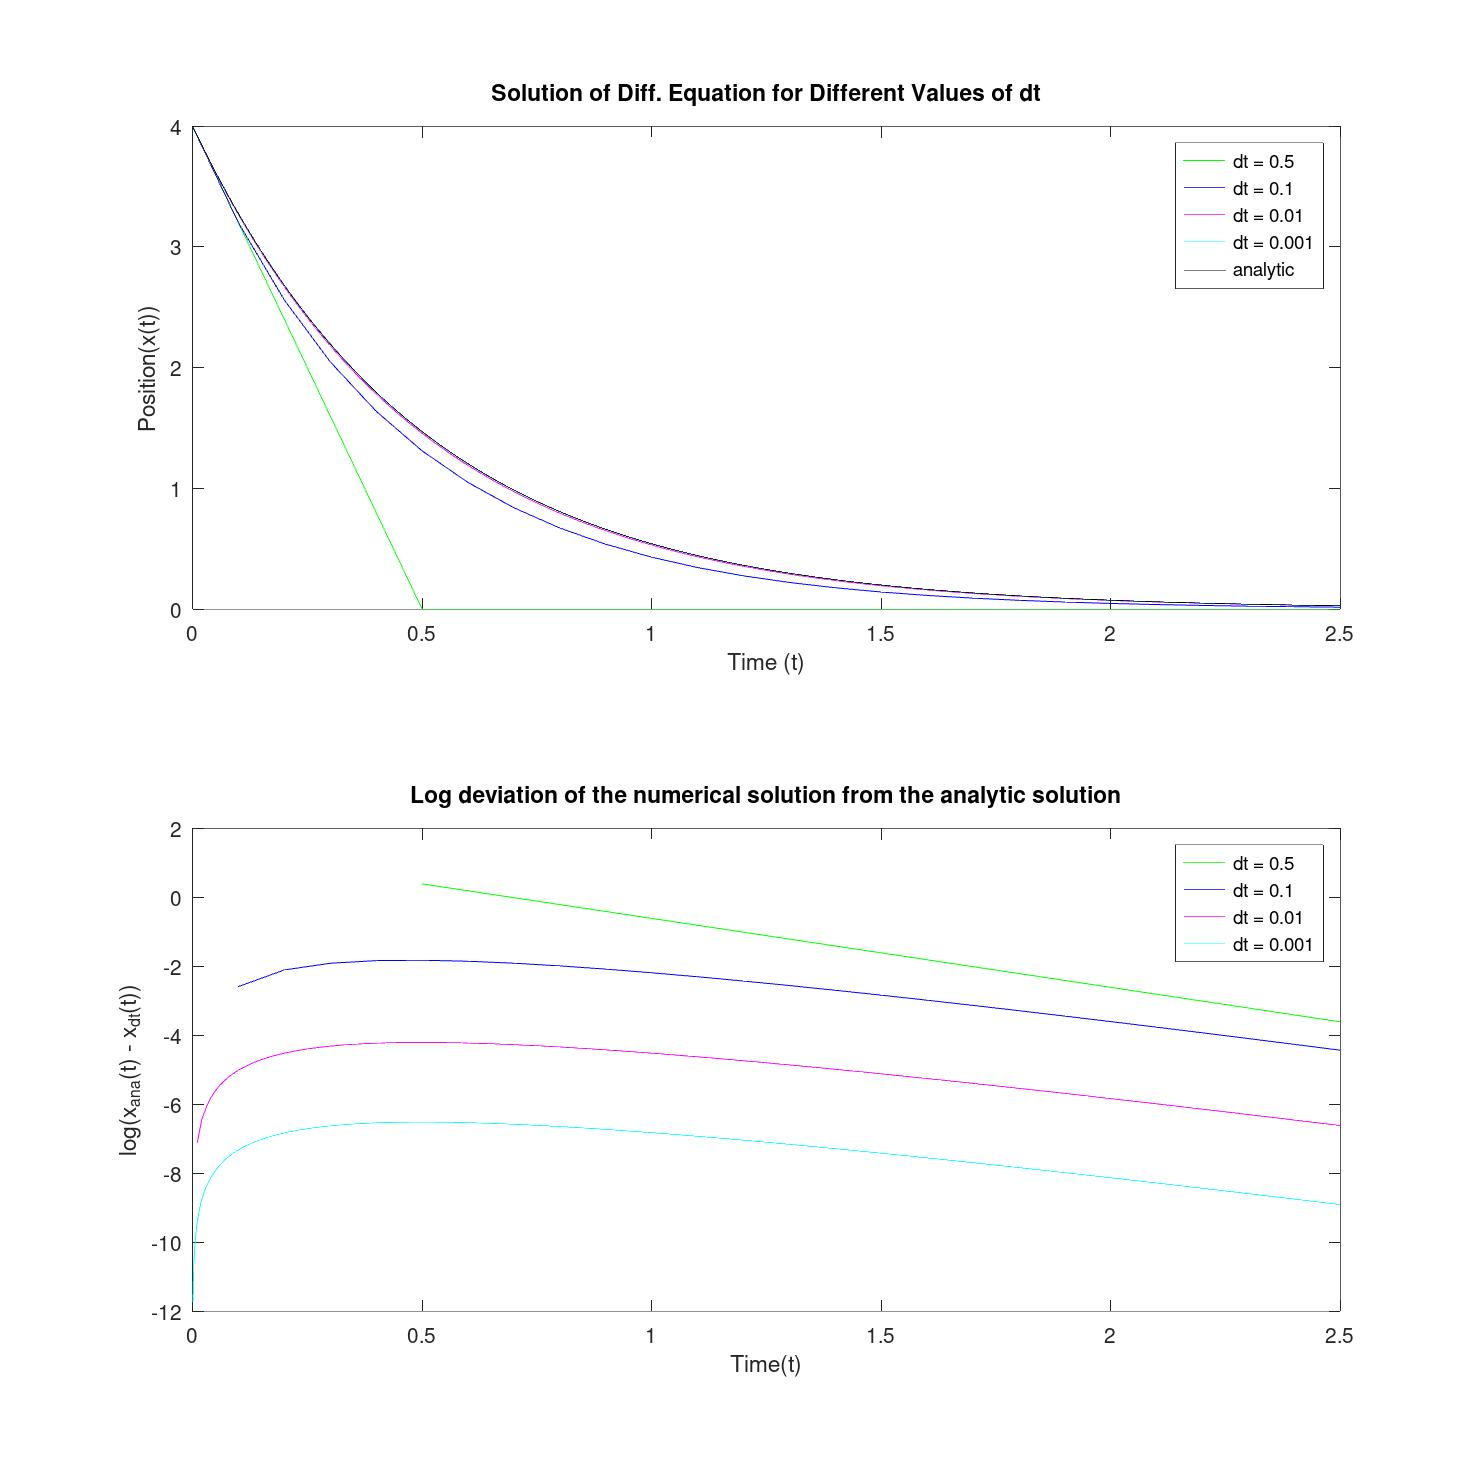
\includegraphics[width=0.75\textwidth]{a2.jpg}
    \caption{Numerical solutions for different $\Delta t$ compared with the analytical solution.}
\end{figure}

\section*{Conclusion}
The Euler method successfully approximates the solution of the differential equation. However, the accuracy depends strongly on the time step $\Delta t$. Larger $\Delta t$ values produce significant deviation, while smaller $\Delta t$ values converge towards the exact solution. The error plots clearly demonstrate the improvement in accuracy with smaller step sizes.
